\chapter{Stand van zaken}
\label{ch:stand-van-zaken}
% Tip: Begin elk hoofdstuk met een paragraaf inleiding die beschrijft hoe
% dit hoofdstuk past binnen het geheel van de bachelorproef. Geef in het
% bijzonder aan wat de link is met het vorige en volgende hoofdstuk.

% Pas na deze inleidende paragraaf komt de eerste sectiehoofding.
In dit hoofdstuk gaan we Kafka en RabbitMq bespreken. Want natuurlijk zijn de begrippen zoals \emph{Kafka} en \emph{RabbitMq} niet voor iedereen even duidelijk. Ook de term microservices zal bij sommigen de wenkbrauwen wel eens doen fronsen. In dit hoofdstuk is het de bedoeling uit te leggen wat al deze begrippen betekenen. Na dit hoofdstuk zul je dankzij deze uitleg in staat zijn om om alles goed te begrijpen.
\section{Microservices}

Microservices is een software architectuur. De applicatie bestaat uit meerdere kleinere microservices die samen één groot geheel vormen. Deze kleinere microservices zijn onafhankelijk van elkaar en hebben elk hun eigen proces. Deze software architectuur is vrij recent en is de laatste jaren een echte hype aan het worden.

Een belangrijke vraag is: waarom zijn microservices ontstaan? Server-side applicaties gebruiken meestal object-georiënteerde programmeertalen. Deze programmeertalen hebben abstracties om de complexiteit van hun programma's te behandelen in modules. Dit wordt ook wel eens `the monolith` genoemd. Dit is één groot geheel dat meestal uit drie lagen bestaat. De presentatielaag, de businesslaag en de datalaag. Deze lagen kunnen niet apart van elkaar gebruikt worden omdat ze verschillende resources met elkaar delen. Dit zorgt ervoor dat bij iedere wijziging in de applicatie, alle lagen opnieuw gereleased worden in een nieuwere versie. Je kan natuurlijk al raden dat dit in een grote applicatie niet de beste oplossing is. 

\begin{figure}[h!]
    \centering
    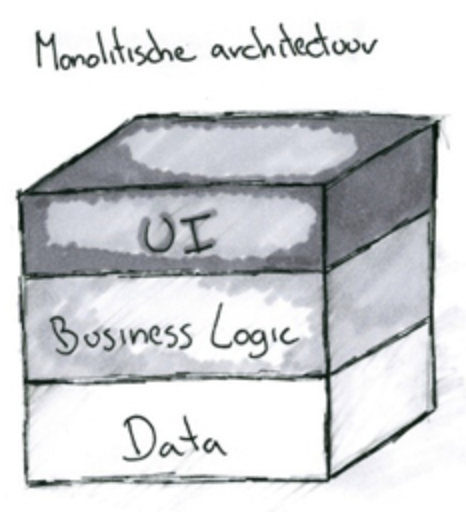
\includegraphics[width=80mm]{../monolith.png}
    \caption{Monolitische architectuur}
        
\end{figure}

Daarom is er een andere architectuur die een heel andere aanpak heeft, namelijk microservices. Dit bestaat uit verschillende kleinere componenten die indien nodig onafhankelijk van elkaar uitgevoerd kunnen worden. Bij deze aanpak is het ook belangrijk dat je uw services klein houdt. Hierdoor kunnen je services gemakkelijk hergebruikt, begrepen en opnieuw gebuild worden. Iedere microservice heeft dus maar 1 verantwoordelijkheid.

Omdat microservices op verschillende machines moeten kunnen draaien, bijvoorbeeld op verschillende besturingssystemen, is het beter om ze in te pakken samen met hun dependencies in een container. \emph{Docker} is een voorbeeld van een technologie die deze containers aanbiedt. Door microservices in containers te plaatsen, zorg je ervoor dat de uitvoering van deze services onafhankelijk gebeurt van andere applicaties op dezelfde machine. Containers zijn dus onafhankelijk van een besturingssysteem, hierdoor kunnen microservices op verschillende locaties gedraaid worden. Een van de voordelen hiervan is dat ze door containers gemakkelijker met de cloud kunnen werken. Een ander voordeel is dat iedere microservice zijn eigen verantwoordelijkheid heeft. Omdat ze maar één verantwoordelijkheid hebben, kunnen ze beter garanderen dat dit ook goed uitgevoerd wordt. Een nadeel van microservices is dat het steeds over het netwerk loopt. Er kan hierdoor vertraging zijn, maar er kan ook iets fout lopen over het netwerk waardoor er mogelijks informatie verloren gaat. Het is nooit de bedoeling dat informatie verloren gaat natuurlijk. Je kan hiervoor maatregelen nemen zodat de kans dat dit gebeurt minimaal is. Een ander nadeel is dat als je veel microservices hebt en die moeten allemaal met elkaar communiceren, dan mag er niets mis zijn met het netwerk om elkaar te vinden. Dit probleem kan opgelost worden door service discovery. Dit is het vinden van de netwerk locatie van een ander microservice. Indien een service een dynamische ip-adres geeft, is het niet de bedoeling dat twee services niet meer met elkaar kunnen communiceren indien een ip-adres verandert. Indien je meer wilt weten over de werking van service discovery dan verwijs ik u graag door naar het artikel van \textcite{Xu2019}.

De vier grootste voordelen van microservices zijn: 
\begin{itemize}
    \item Schaalbaarheid
    \item Beperken complexiteit
    \item Verkorten time-to-market
    \item Autonomie van ontwikkelteams: je kan met verschillende teams werken, je kan de beste technologie kiezen, afhankelijk van het probleem dat je wilt oplossen.
\end{itemize}

\emph{Kafka}, \emph{RabbitMq} en \emph{Google Pub/Sub} zijn technologieën die gebruikt kunnen worden om informatie te verwerken in microservices. Hieronder verklaren we hoe deze verschillende technologieën werken en waar de verschillen zitten.

 \autocite{Claudio2017}, \autocite{Velthoven2016} en \autocite{Xu2019}

\section{Kafka}

Wanneer je als bedrijf veel berichten binnen krijgt op een korte tijdsspanne, dan heb je natuurlijk een goed functionerende technologie nodig die al deze berichten kan verwerken. \emph{Kafka} is een voorbeeld van zo een technologie. Het is dus een berichtensysteem waarbij schaalbaarheid en redundantie een grote troef zijn. Bepaalde kernwoorden zijn belangrijk om de architectuur van \emph{Kafka} te begrijpen. Deze kernwoorden zijn: topics, producers, consumers en brokers.  

Als producer kun je een bericht verzenden naar uw gewenste topic. Topics zijn, zoals de naam al doet vermoeden, verschillende onderwerpen. Alle berichten zijn gegroepeerd in een van deze topics. Een topic kan verschillende nodes hebben, maar het kan ook zijn dat er maar één node is. Als er verschillende nodes zijn dan kan je de inkomende data repliceren. Een node kan opgedeeld zijn in verschillende partities. Als een bericht binnenkomt, dan wordt deze opgeslagen in een partitie van je topic die op zijn beurt weer op een verschillende node kan zitten.

Een topic kan je dus verdelen in verschillende partities. Dit wil zeggen dat je uw data kunt verdelen in ongeveer gelijke groepen. Iedere partitie kan dan staan voor een specifieke groep data binnen een topic zodat je niet alle berichten altijd moet overlopen. Dit principe van verschillende partities wordt ook gebruikt bij traditionele databanken. Het is dus geen garantie dat het effectief gelijke groepen zijn. De bestemming van een bericht hangt af van de message-key. Als je bijvoorbeeld woorden wilt groeperen en je verdeelt je groepen volgens de eerste letter van ieder woord. Dan staan alle woorden die beginnen met een a samen, ieder woord dat begint met een b, ... Als je dan toevallig veel woorden binnen krijgt die beginnen met een c, dan kan het gebeuren dat je groepen niet gelijk verdeeld zijn.

Een bericht heeft een bepaalde retention. Dit is de tijd dat het bericht maximum beschikbaar is. Als bijvoorbeeld de retention op zeven dagen staat, en je binnen deze zeven dagen het bericht niet gelezen hebt, dan wordt het bericht verwijderd. Dan is het niet meer mogelijk om de inhoud van het bericht nog ooit op te vragen. Het formaat van een bericht kan verschillend zijn. Het type kan een gewone tekst zijn, kan van een Json-formaat zijn, of kan iets helemaal anders zijn. Dit waren allemaal voorbeelden van leesbare data, maar het is ook mogelijk dat het niet leesbaar is. Het formaat kan ook binair zijn, Avro is hier een voorbeeld van. Het is mogelijk om zowel naar een specifieke topic een bericht te verzenden als te ontvangen. 

Dit brengt ons naadloos bij het volgende begrip: consumers. Een consumer kan zelf bepalen van welke topic hij berichten wilt ontvangen. Consumers binnen een consumer-groep worden automatisch enkele partities toegewezen. Door topics en consumers op deze manier op te delen, zorg je ervoor dat het mogelijk is dat meerdere consumers kunnen lezen van meerdere partities in een topic. Dit heeft als positief gevolg dat je meer berichten kunt verwerken binnen een bepaalde tijd. Het is al even vermeld, maar wat is nu eigenlijk een consumer-groep? Dit is een verzameling van verschillende consumers. Iedere consumer op zich leest van één specifieke partitie waardoor je het aantal verwerkte berichten binnen één tijdseenheid kunt verhogen. Alle consumers binnen één groep lezen samen alle berichten die op een topic staan. Het opdelen van je topic in verschillende partities zorgt er dus niet voor dat je een deel van je data verliest. Mochten er meer consumers zijn dan dat er partities zijn, dan zitten er sommigen zonder werk. Omgekeerd, als er meer partities zijn dan consumers, dan krijgen consumers van verschillende partities berichten binnen. De hoeveelheid consumers binnen een groep is afhankelijk van de hoeveelheid partities die er zijn.

 \begin{figure}[h!]
    \centering
    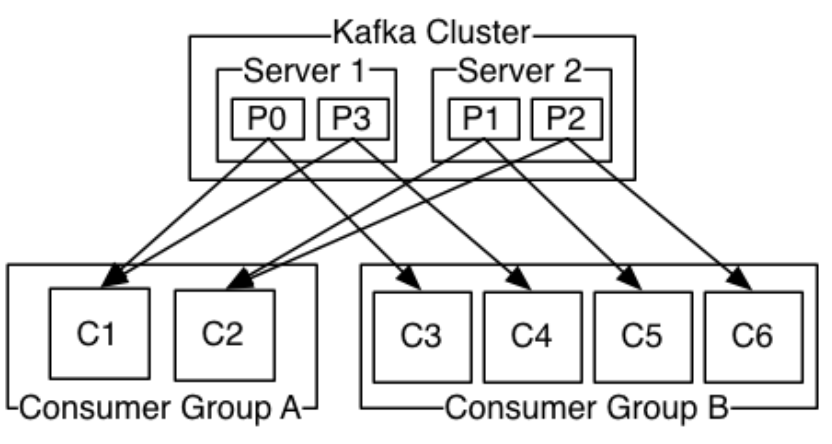
\includegraphics[width=80mm]{../kafkaConsumers.png}
    \caption{Wisselwerking tussen partities en consumer-groepen, \autocite{Sookocheff2015}}
    
\end{figure}

Figuur 2.2 is een voorbeeld hoe een topic in verschillende servers kan opgedeeld worden en hoe consumers in consumer-groepen kunnen onderverdeeld worden. Je ziet dat de Kafka cluster in twee servers onderverdeeld is. Iedere server heeft twee partities. Er zijn 2 consumer-groepen, groep A bestaat uit twee consumers, groep B bestaat uit 4 consumers. Iedere partitie kan dus naar verschillende consumer-groepen berichten versturen, maar kan niet binnen dezelfde consumer-groep naar een andere consumer iets verzenden. 

Het laatste woord dat nog moet verduidelijkt worden is een broker. \emph{Kafka} draait op een cluster. Iedere cluster bestaat uit één of meerdere nodes(servers). Per Kafka cluster kunnen er verschillende producers en consumers zijn, zoals te zien is op figuur 2.3. 

\begin{figure}[h!]
    \centering
    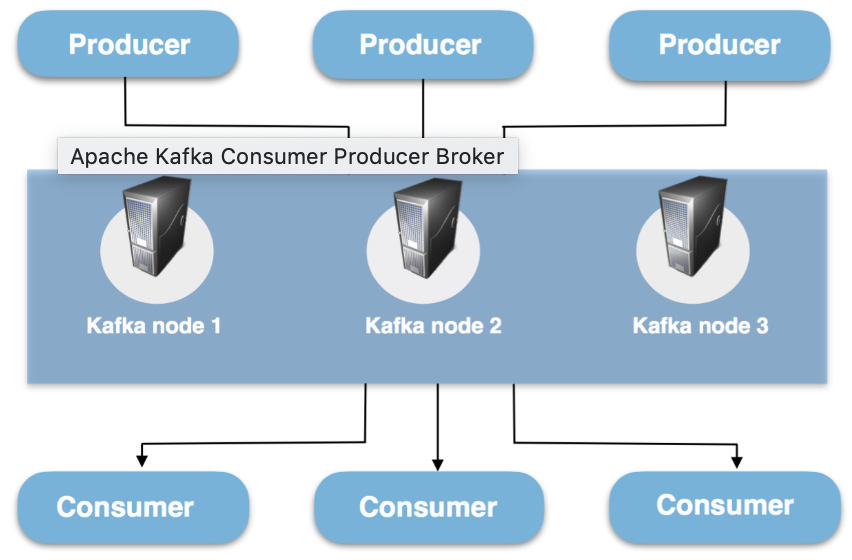
\includegraphics[width=80mm]{../kafkaCluster.png}
    \caption{Voorbeeld van een Kafka cluster, \autocite{Johansson2016}}
    
\end{figure}


 Ieder bericht binnen een partitie heeft een offset. Dit is een identifier, waardoor het mogelijk is om de berichten te ordenen. Normaal gezien als je als consumer een subscriptie maakt op een topic, dan krijg je vanaf dit moment alle nieuwe berichten die binnen komen op de partitie waarop je een subscriptie hebt. Door een offset is het mogelijk om iets oudere berichten die op een partitie staan dan het moment dat je een subscriptie aangemaakt hebt, ook op te vragen. Op figuur 2.4 zie je een simpele voorstelling van een producer die berichten op een partitie van een topic plaatst. De cijfertjes stellen de offset voor van een bericht.
 \begin{figure}[h!]
     \centering
     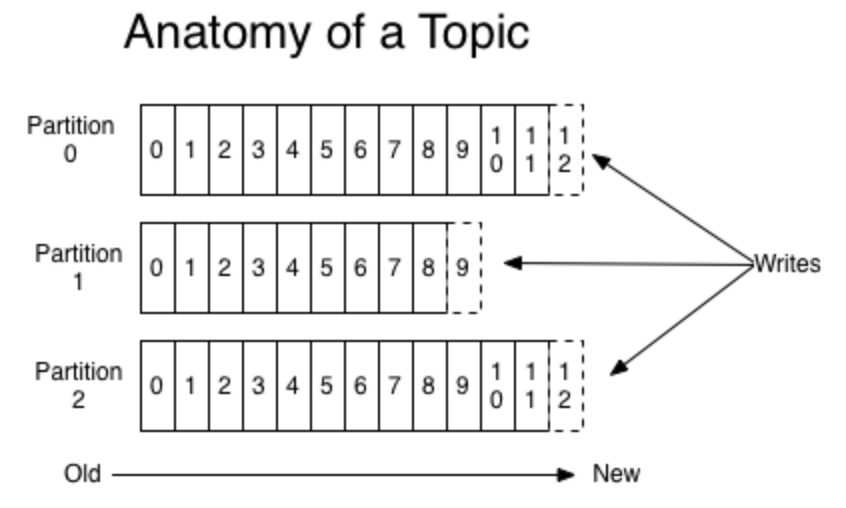
\includegraphics[width=80mm]{../kafkaOffset.png}
     \caption{Simpele voorstelling van de werking van een offset, \autocite{Sookocheff2015}}
     
 \end{figure}


\autocite{Sookocheff2015} en \autocite{Johansson2016}

\section{RabbitMq}

Een alternatief voor \emph{Kafka} is \emph{RabbitMq}. Dit is software waar men berichten kan plaatsen en ophalen op één of meerdere 'queues'. Ook hier heb je verschillende mogelijkheden van wat het formaat is van de berichten. Het kan zowel een gewone tekst zijn, als een Json-file. 

Er zijn hier ook producers die data op de queue zetten, alsook consumers die een binding kunnen maken op een queue. Wanneer een bericht van een queue wordt gelezen, dan wordt deze verwijderd van de queue. Het is dus niet mogelijk om later opnieuw hetzelfde bericht op te gaan vragen. 

\emph{RabbitMq} kan een voordeel zijn om te gebruiken in verschillende situaties. Als je bijvoorbeeld als gebruiker de data die je opslaat in een queue wilt distribueren naar verschillende consumers, dan is ook \emph{RabbitMq} een ideale technologie om dit te doen. Het is dus mogelijk dat verschillende consumers de berichten lezen. Een ander voordeel is dat het mogelijk is om je berichten te verdelen over verschillende consumers. Op deze manier wordt dan de hoeveelheid mooi gebalanceerd verdeeld over de verschillende consumers.

Een broker bij \emph{RabbitMq} is de exchange en de queues. De exchange is verantwoordelijk voor het verzenden van de berichten naar de verschillende queues. Indien een bericht in de broker toekomt, moet deze dus eerst langs de exchange voordat hij in een queue terecht kan. De link tussen de queue en de exchange wordt ook wel eens een binding genoemd.

Er zijn vier verschillende soorten van exchanges. Dit zijn: direct, fanout, topic en headers exchanges. Drie van deze worden uitgebeeld in figuur 2.5 \begin{itemize}
    \item De direct exchanges sturen berichten naar een queue op basis van een routing key. Deze key is hetzelfde als de binding key van de queue waarnaar het naartoe moet verzenden. 
    \item Fanout exchanges sturen berichten naar alle queues die verbonden zijn met de exchange
    \item Bij Topic exchanges worden wildcard matches gebruikt . De match wordt gedaan tussen de routing key en de routing pattern die in de binding gespecificeerd wordt.
    \item Header exchanges gebruiken de attributen uit de header om te bepalen welke queue de bestemming is van een bericht.
\end{itemize}
 \begin{figure}[h!]
    \centering
    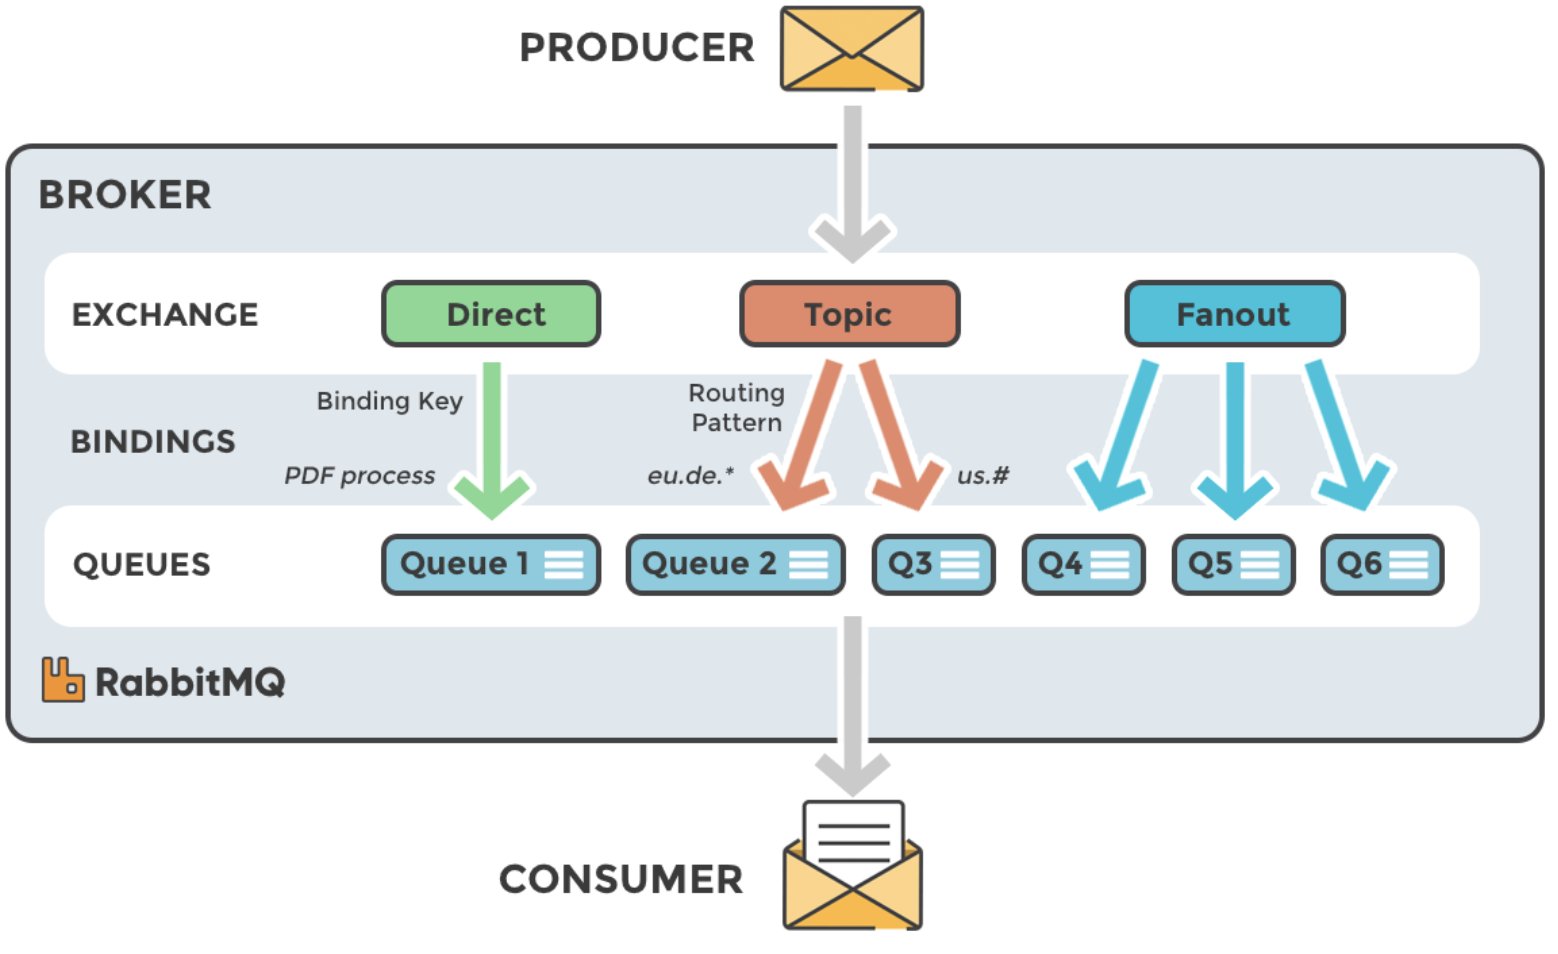
\includegraphics[width=60mm]{../rabbitmqExchanges.png}
    \caption{Werking drie verschillende exchanges bij \emph{RabbitMq}, \autocite{Johansson2015}}
    
\end{figure}
\autocite{Johansson2015}
\section{Kafka vs RabbitMq}
Als we kijken naar Google Trends om te bepalen welke van deze twee technologiën nu het populairste is, dan krijgen we in figuur 2.6 een grafiek te zien van het afgelopen jaar.
 \begin{figure}[h!]
    \centering
    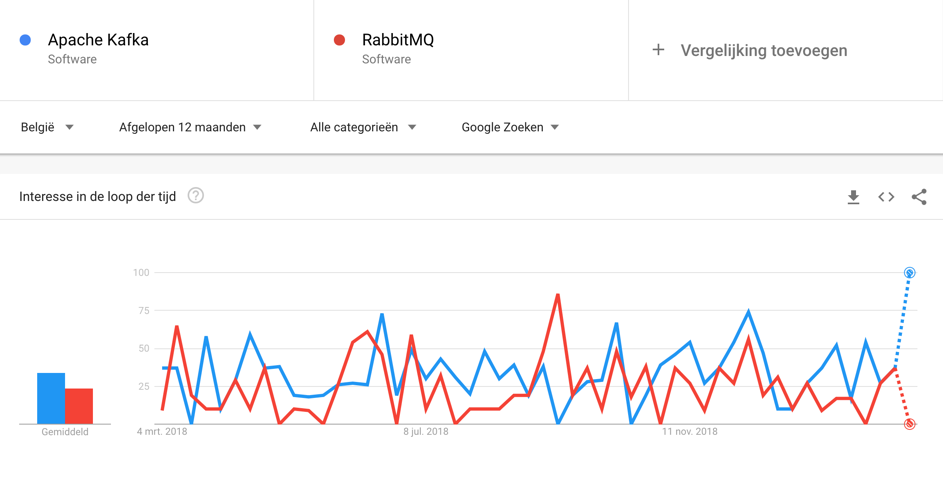
\includegraphics[width=100mm]{../KvsRMQ1.png}
    \caption{Populariteit \emph{Kafka} en \emph{RabbitMq} in het afgelopen jaar, \autocite{Trends2019}}
    
\end{figure}

In deze grafiek is duidelijk te zien dat \emph{Kafka} iets populairder is dan \emph{RabbitMq}. Er zit tussen juli en november wel een piek in waarbij \emph{RabbitMq} veel populairder is, maar over het algemeen gezien kunnen we concluderen dat in het afgelopen jaar \emph{Kafka} toch iet wat populairder is.

 \begin{figure}[h!]
    \centering
    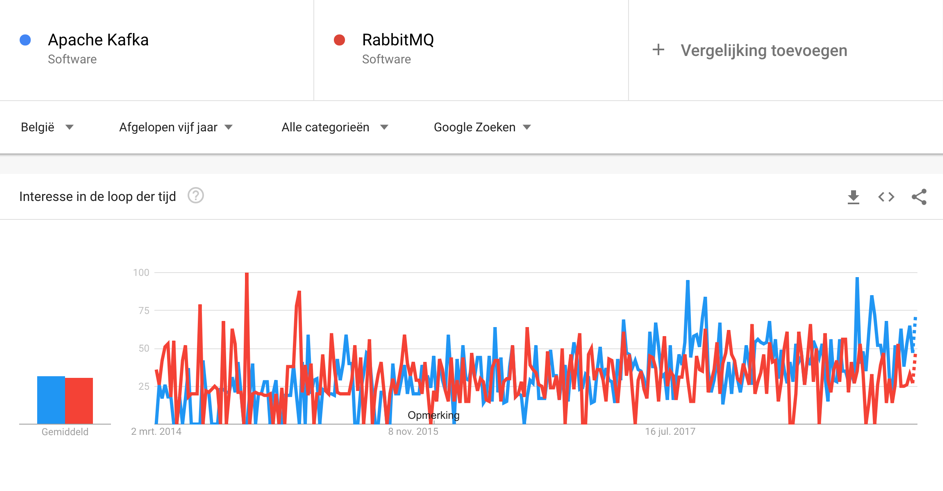
\includegraphics[width=100mm]{../KvsRMQ2.png}
    \caption{Populariteit \emph{Kafka} en \emph{RabbitMq} in de afgelopen vijf jaar, \autocite{Trends2019}}
    
\end{figure}

Als je figuur 2.7 bekijkt, dan zie je een algemene trend. Namelijk dat vijf jaar geleden \emph{RabbitMq} veel populairder was, maar dat deze trend systematisch omgedraaid is. Uit deze figuur valt ook af te leiden dat in het algemeen de interesse naar technologieën voor microservices lichtjes toegenomen is in de laatste vijf jaar.

\autocite{Trends2019}

\section{Google Pub/Sub}
Tijdens het academiejaar dat dit onderzoek is uitgevoerd, zijn de gebruikte technologieën die TVH gebruikt ook wat veranderd. Er is momenteel een nieuwe technologie bij gekomen, namelijk \emph{Google Pub/Sub}. Zoals de naam doet vermoeden is Google eigenaar van deze technologie. 

Ook hier zijn het ongeveer dezelfde kernwoorden die belangrijk zijn:
\begin{itemize}
    \item Topic
    \item Subscription
    \item Message
    \item Publisher
    \item Subscriber
\end{itemize}

De termen topic en message zijn hetzelfde als bij de andere technologieën. Subscription is de link tussen de subscriber (deze wordt straks uitgelegd), en de topic. Dit is dus een soort van abonnement die een subscriber aangaat met een topic. Een subscriber is iemand of iets die de verschillende messages van een specifieke topic leest. Een publisher is dan degene die nieuwe messages op een topic plaatst.

 \begin{figure}[h!]
    \centering
    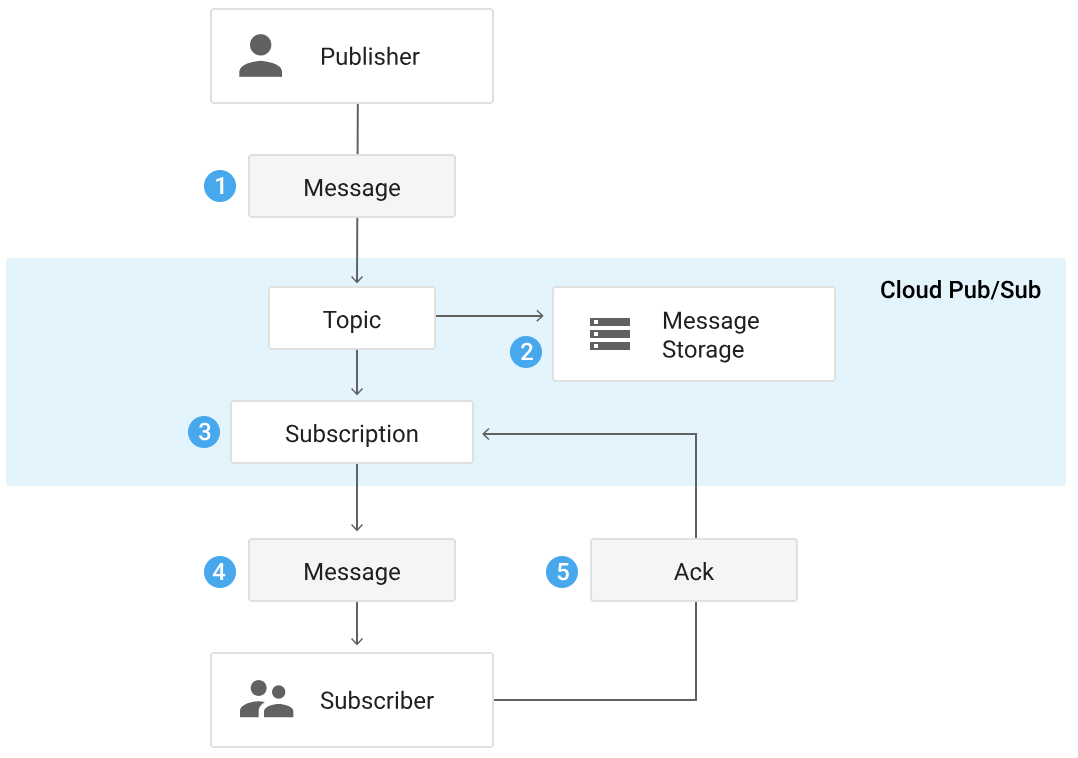
\includegraphics[width=100mm]{../gpsFlow.png}
    \caption{De flow die een message aflegt bij \emph{Google Pub/Sub}, \autocite{Google2019}}
    
\end{figure}

Op figuur 2.8 is te zien hoe een message tot bij een subscriber geraakt, iemand of iets die de message leest. Eerste stap is de publisher die een message plaatst (published) naar een topic. Een message bevat een payload, dit is de inhoud van de message. Ook kan er eventueel attributen toegevoegd worden die iets meer vertellen over de inhoud van de payload. Vervolgens wordt in de tweede stap de message opgeslagen in de Message Storage totdat een subscriber de message leest en acknowledged. Dit wil zeggen dat de subscriber een bevestiging stuurt naar de subscription om te melden dat hij de message goed ontvangen heeft. Hierna zet de Pub/Sub deze message klaar in al zijn subscriptions. Deze message wordt dan gelezen als bijvoorbeeld de subscriber deze message binnen trekt. In de vierde stap zien we dat alle berichten die nog niet gelezen zijn door de subscriber, bij de subscriber binnen komen. Als een message goed is aangekomen, dan wordt er een acknowledge gestuurd naar de subscription. Dan wordt deze message ook verwijderd en kan deze niet meer opnieuw gelezen worden. Dit is de vijfde stap.

\autocite{Google2019}

\section{IoT-applicatie}
Microservices architectuur wordt meestal gebruikt in een IoT-applicatie. Bij microservices is het meestal zo dat er veel data is. En bij IoT wordt er veel data verzonden. Voluit staat IoT voor Internet of Things. Onder deze noemer verstaan we machines en alledaagse objecten die verbonden staan met het internet en eventueel ook met elkaar.

Iedereen weet wat de voordelen zijn van internet op toestellen zoals een gsm, tablet, ... Laten we naar het voorbeeld van een gsm bekijken. Als je vergelijkt wat een gsm allemaal kon toen er nog geen internet mogelijk was en nu, dan zie je dat het eigenlijk een ander toestel geworden is met veel meer functionaliteiten. Dit is ook zo bij alledaagse objecten. Met het toevoegen van internet op deze objecten verhoog je de functionaliteit ervan. We zullen dit even illustreren met een voorbeeldje. Neem nu een lamp in je woonkamer. Dankzij IoT ben je niet meer verplicht om manueel een schakelaar die fysiek aanwezig is in je woonkamer om te draaien. Door de lamp te verbinden met het internet kan je die ook vanop afstand aan of uit schakelen via een app op je smartphone of iets dergelijks. Dit geeft extra voordelen aan het product. Als we ons eigen voorbeeldje nog een bekijken, kan dit handig zijn als je vergeten het licht te doven bent indien je bijvoorbeeld naar je werk vertrokken bent. Dan neem je gewoon je smartphone en doof je het licht vanop afstand. Zonder IoT was dit allemaal niet mogelijk geweest.

 \begin{figure}[h!]
    \centering
    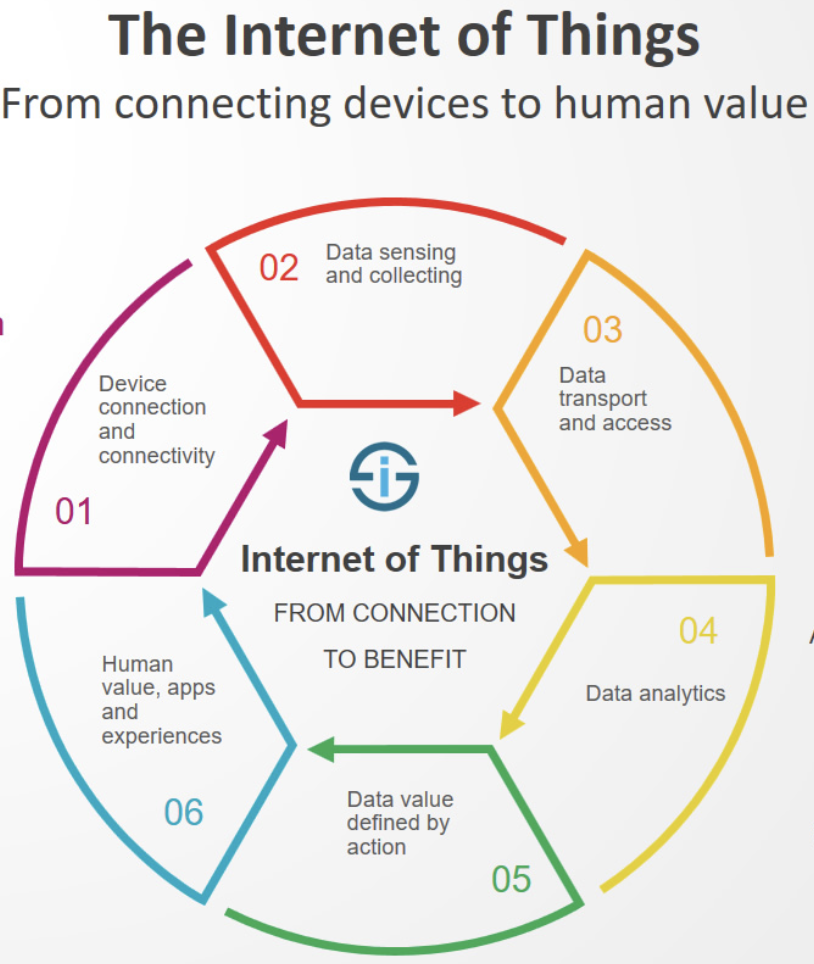
\includegraphics[width=65mm]{../IoT.png}
    \caption{De gecreëerde waarde van IoT, \autocite{i-scoop2019}}
    
\end{figure}

Op figuur 2.9 kan je de flow zien hoe Internet of Things extra waarde oplevert voor een bedrijf. In de eerste stap zorg je ervoor dat je object waar je informatie uit wilt halen verbonden is met het internet. Vervolgens worden er metingen en waarnemingen gedaan zodat er iets is dat het toestel kan verzenden. Nadien wordt de data natuurlijk effectief verzonden. Als vierde stap kan je eventueel analyses doen op je verkregen informatie zodat je nog extra zaken kunt concluderen. In de volgende stap moet je natuurlijk waarde hechten aan de informatie die binnen komt. Want natuurlijk weet het apparaat dat informatie verstuurt niet waarvoor een bepaald cijfer staat. De bedoeling in deze stap is dus bepaalde waarde voor het bedrijf toevoegen aan de verkregen getallen of waarden. Als laatste stap kan je conclusies trekken en eventueel zelf als bedrijf mogelijke acties ondernemen. Deze 6 stappen illustreren hoe je door het toevoegen van connectiviteit extra waarde voor een bedrijf kunt realiseren.

Het is nu niet zo dat alleen alles wat je van op afstand aan of uit kunt schakelen onder de noemer IoT valt. Er zijn voornamelijk drie categorieën waarin we Internet of Things objecten onderscheiden.

\begin{itemize}
    \item Zaken die informatie verzamelen en verzenden.
    \item Zaken die informatie verzamelen en daaropvolgend een actie uitvoeren.
    \item Zaken die de twee bovenstaande combineren.
\end{itemize}

Het bedrijf TVH gebruikt voornamelijk de eerste categorie. Dit wordt in 2.7 uitgelegd.

\subsection{Informatie verzamelen en verzenden}
Bij deze categorie komen er sensoren bij kijken. Sensoren kunnen van verschillende type zijn: bewegins-, temperatuur- of lichtsensoren bijvoorbeeld. Alle mogelijke types van sensoren kunnen hiervoor gebruikt worden. Deze sensoren zijn verbonden met het internet en nemen bepaalde waarnemingen aan van de omgeving. Deze waarnemingen zijn afhankelijk van het type sensor. Bijvoorbeeld bij een temperatuursensor zal deze om een bepaalde tijd de temperatuur van zijn locatie verzenden. De informatie die sensoren verzenden kunnen van grote waarde zijn voor bedrijven. Hierdoor kunnen ze bepaalde beslissingen nemen die mogelijk tot meer winst of andere voordelen leiden. 

\subsection{Informatie verzamelen en reageren}
De voorbeelden van deze categorie liggen dichter bij de hand dan je zou denken. Er zijn tal van voorwerpen die dagelijks gebruikt worden die informatie verzamelen en erop reageren. Enkele voorbeelden zijn: een printer die een document ontvangt en uitprint of een autosleutel die je auto open maakt of sluit wanneer je op het juiste knopje duwt.

Deze voorbeelden zorgen niet meteen voor een business-waarde om bijvoorbeeld de winst van een bedrijf te verhogen. Dit wilt niet zeggen dat deze zaken daarom minder interessant zijn.

\subsection{Combinatie}
Door deze twee categorieën te combineren, krijgen we nieuwe mogelijkheden. Door deze combinatie kun je een voortdurende wisselwerking creëren tussen acties die iemand neemt en de reacties die het object maakt. Laten we een fictief voorbeeldje verzinnen. Stel je wilt een cilindervormig voorwerp vullen met water. Het voorwerp kan 100 liter water bevatten. De bedoeling is dat het water altijd tussen de 80 en 90 liter moet blijven. Dan kan je een sensor installeren die detecteert of het water onder de 80 liter zit. Indien de sensor dit detecteert, moet hij automatisch het voorwerp bijvullen. De machine stopt met het object te vullen wanneer de sensor detecteert dat hij aan 89 liter zit. Hierop voert hij een actie uit om geen water meer bij te vullen. Op deze manier is er een continue werking van het systeem door het verzamelen van informatie en een actie uit te voeren aan de hand van de ontvangen informatie. Voor veel bedrijven kan dit handig zijn om processen te optimaliseren, want er moeten in principe geen mensen meer aan de pas komen. Vroeger zou in dit voorbeeldje een mens voortdurend handmatig controleren of het water niet onder de 80 liter zat, daarna zelf het voorwerp bijvullen. Hierbij was er nog een extra risico dat de persoon te laat ontdekt dat er meer dan 90 liter water zou zijn. Dit zou erge gevolgen kunnen hebben voor een bedrijf.

\autocite{McClelland2019} en \autocite{i-scoop2019}

\section{TVH}
Dit onderzoek wordt uitgevoerd ten voordele van het bedrijf TVH. Dit is een familiebedrijf die oorspronkelijk opgericht is door Paul Thermote en Paul Vanhalst. Ze begonnen in een schuur waar ze kapotte landbouwmachines en forklifts repareerden. Later begonnen ze ook met het verkopen van deze machines. Dit bestond voornamelijk uit het repareren van tweedehands machines en het verkopen ervan. Vervolgens begonnen ze snel met het verhuren van deze werktuigen. Nog enkele jaren later begonnen ze met de verkoop van vervangonderdelen voor machines. Nadien werden er nog een paar bedrijven overgenomen waardoor het bedrijf uitgroeide tot het grote bedrijf dat we vandaag de dag kennen. 

Maar wat is het nut nu van dit onderzoek voor TVH? Zoals je overal ziet, is internet bijna nergens meer weg te denken. Ook voor dit bedrijf kan internet enkele voordelen bieden. Zoals eerder vermeld in de sectie over IoT-applicatie gebruikt TVH vooral de eerste categorie, namelijk het verzamelen van informatie en het verzenden ervan.

Aan ieder werktuig hangt een tracking-device. Met dit toestel is het mogelijk om de locatie van al hun toestellen die ze verhuren te lokaliseren. Maar deze apparaten verzenden niet alleen hun locatie, ze verzenden ook veel andere nuttige informatie. Ze houden bijvoorbeeld bij hoeveel werkuren een machine al bezig is. Of ze sturen door als de motor van de machine aanligt, de machine aan het bewegen is, ... Kort samengevat: er komt heel veel informatie binnen uit deze toestellen en daar zit heel veel handige informatie in voor het bedrijf. Zo kunnen ze bijvoorbeeld na een tijdje te weten komen wat de tijd is tot dat een onderdeel van een machine vervangen moet worden. Of ze kunnen bedrijven die machines huren controleren dat ze effectief alleen de werktuigen gebruiken tijdens de werkweek, en niet tijdens het weekend.

Laten we nog even figuur 2.9 erbij nemen. We hebben al algemeen uitgelegd wat deze afbeelding voorstelt. Nu gaan we dit even toepassen op het bedrijf TVH. In de eerste stap worden de tracking-devices aan de werktuigen gekoppeld. Nadien verzamelen deze devices informatie over de machines. Deze informatie wordt dan in stap drie verzonden. Een voorbeeld van analyse op de informatie die binnenkomt binnen het bedrijf is controleren als het tracking-device dat informatie verzendt wel gekoppeld is aan een werktuig. In stap vijf koppel je de cijfers aan specifieke waarden. Bijvoorbeeld input 2 geeft 0 of 1 terug. Dit kan betekenen dat een motor van een machine al dan niet aanligt. In de laatste stap kan het bedrijf effectief acties ondernemen uit de conclusies die getrokken kunnen worden van de verkregen informatie.

Dankzij de tracking-devices zijn alle machines gekoppeld aan het internet. Voor een IoT-applicatie die al deze informatie verzamelt heb je natuurlijk een goede technologie nodig. \emph{Kafka}, \emph{RabbitMq} en \emph{Google Pub/Sub} zijn mogelijke technologieën en zijn al reeds uitgelegd. Dit onderzoek moet uitwijzen welke technologie het beste is voor TVH om deze informatie te verzamelen.



